\chapter{Convex Hull}
\section{Introduction}
Given a set of points in the plane. the convex hull of the set is the smallest convex polygon that contains all the points of it. There are many different algorithms to find the convex hull. We will mainly focus on the two most famous ones : Jarvis March and Graham's scan.  

\section{Right Hand Thumb Rule}
\begin{wrapfigure}{R}{0.3\textwidth}
\centering
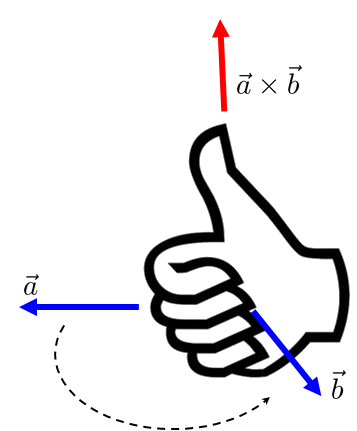
\includegraphics[width=0.25\textwidth]{images/rhtr.png}
\caption{\label{fig:frog1}Right hand thumb rule}
\end{wrapfigure}

The conventional criterion for right-handedness of screws is to curl your right hand's fingers around it while running your thumb along it. It's right-handed if it screws in (in the direction of your thumb) when twisted in the direction your fingers point.

The right hand rule for rotation vectors works on the same principle: curl your right hand's fingers in the rotation's direction. If it isn't possible, rotate your wrist until it is. The rotation vector is then determined by the direction of your thumb.

Anyways, why do we need this? We will very soon realize that we need some tool to get a sense of clockwise and anticlockwise directions to find the convex hull. We say that the angle is clockwise if cross product is positive, while anticlockwise if its negative. In other words, if we want to go from $\vec{a}$ to $\vec{b}$ and $\vec{a} \times \vec{b}$ is positive, then we have to go clockwise, else anticlockwise. \clearpage
\section{Template}
We will use the below template for convex hull, and any other geometry problem later.
\begin{minted}
[
frame=lines,
framesep=2mm,
baselinestretch=1.2,
fontsize=\footnotesize,
linenos
]
{cpp}
template <class T> int sgn(T x) { return (x > 0) - (x < 0); }
template<class T>
struct Point {
	typedef Point P;
	T x, y;
	explicit Point(T x=0, T y=0) : x(x), y(y) {}
	bool operator<(P p) const { return tie(x,y) < tie(p.x,p.y); }
	bool operator==(P p) const { return tie(x,y)==tie(p.x,p.y); }
	P operator+(P p) const { return P(x+p.x, y+p.y); }
	P operator-(P p) const { return P(x-p.x, y-p.y); }
	P operator*(T d) const { return P(x*d, y*d); }
	P operator/(T d) const { return P(x/d, y/d); }
	T dot(P p) const { return x*p.x + y*p.y; }
	T cross(P p) const { return x*p.y - y*p.x; }
	T cross(P a, P b) const { return (a-*this).cross(b-*this); }
	T dist2() const { return x*x + y*y; }
	double dist() const { return sqrt((double)dist2()); }
	double angle() const { return atan2(y, x); }
	bool null() const { return (x == 0 && y == 0); }
	P unit() const { return *this/dist(); } // makes dist()=1
	P perp() const { return P(-y, x); } // rotates +90 degrees
	P normal() const { return perp().unit(); }
	P rotate(double a) const {
		return P(x*cos(a)-y*sin(a),x*sin(a)+y*cos(a)); }
	friend ostream& operator<<(ostream& os, P p) {
		return os << "(" << p.x << "," << p.y << ")"; }
};
\end{minted}
\section{Jarvis March}
This is probably the most obvious non-brute algorithm that most people would come up with.
\begin{figure}[h]
    \centering
    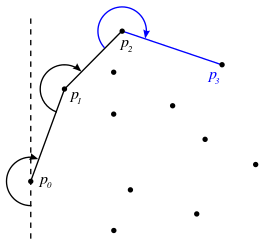
\includegraphics[scale=0.4]{images/jarvis.png}
    \caption{Jarvis Hull}
    \label{fig:my_label}
    
\end{figure}
We start by selecting one point that will definitely be a part of the convex hull. This can be one of the $X$ or $Y$ extremes. Let's say we select the leftmost point. Let's say we want move in a clockwise fashion. So, for any given point, we check for a point which is the leftmost. In other words, if we join the initial and final points, then the cross product of this vector with any other vector (with the same initial point) is non-positive.
The code for this would look as follows:
\begin{minted}
[
frame=lines,
framesep=2mm,
baselinestretch=1.2,
fontsize=\footnotesize,
linenos
]
{cpp}
using P = Point<int>;
vector<P> jarvisMarch(vector<P> pts) {
	int l = 0;
    vector<P>convex_hull;
    for(int i=0; i<pts.size(); i++)
        if(pts[i].y < pts[l].y)
            l = i;
    int pt = l;
    int ch;
    do{
        convex_hull.push_back(pts[pt]);
        ch = (pt+1)%(pts.size());
        for(int i=0; i<pts.size(); i++)
        {
            if((pts[i] - pts[pt]).null())continue;
            if((pts[ch] - pts[pt]).cross(pts[i] - pts[pt]) < 0)
                ch = i;
            else if((pts[ch] - pts[pt]).cross(pts[i] - pts[pt]) == 0)
                if((pts[ch] - pts[pt]).dist() < (pts[i] - pts[pt]).dist())
                    ch = i;
        }
        pt = ch;
    } while (pt != l);
    return convex_hull;
}
\end{minted}
\subsection{Complexity Analysis}
Let's say the convex hull has $m$ edges. Then the worst case time complexity is $O(nm)$. So, if we somehow know that the hull would have less number of edges, then this is a good method. The average time complexity is around $O(n \log n)$. The space complexity is $O(n)$ 

\section{Graham's Scan}
Unless we have any explicit information about the set of points, it's much better to use Graham's Scan algorithm. We will soon realize why. First, we search for the leftmost point. This is because, we are absolutely sure that this point will be a part of convex hull.
\begin{minted}
[
frame=lines,
framesep=2mm,
baselinestretch=1.2,
fontsize=\footnotesize,
linenos
]
{cpp}
using P = Point<int>;
vector<P> GrahamScan(vector<P> pts){
    int l = 0;
    vector<P>convex_hull;
    for(int i=0; i<pts.size(); i++)
        if(pts[i].y < pts[l].y)
            l = i;
    P p = pts[l];
    sort(pts.begin(), pts.end(), [&p](P &a, P &b) {
        if((b-p).cross(a-p) < 0)
            return true;
        else if((b-p).cross(a-p) == 0 && (b-p).dist() > (a-p).dist())
            return true;
        else
        return false;
    });

    convex_hull.push_back(pts[0]);
    convex_hull.push_back(pts[1]);
    P last, second_last;
    for(int i=2; i<pts.size(); i++)
    {
        if((pts[i] -  pts[i-1]).null())continue;
        int sz = convex_hull.size();
        last = convex_hull[sz-1];
        second_last = convex_hull[sz-2];
        while((pts[i] - last).cross(last - second_last) >= 0)
        {
            convex_hull.pop_back();
            sz--;
            last = convex_hull[sz-1];
            second_last = convex_hull[sz-2];
        }

        convex_hull.push_back(pts[i]);
    }
    if(convex_hull[0] == convex_hull[1])
        convex_hull.erase(convex_hull.begin());
    return convex_hull;
} 
\end{minted}

Next, we sort all the points with respect to the angle they make with this point (in clockwise direction). For this, we make a custom comparator function (lines $10$ to $15$). If the angle is $0$ degree, then select the closest point.

First, push the first $2$ points into the stack. Now, iterate through the sorted vector , and do the following : if the old vector (made by last and second last points of stack) and the new vector (made by current point, and last element of stack) is clockwise, then continue. If the condition isn't satisfied, keep popping the last elements off the stack unless the condition is satisfied. While doing all of this, be sure to deal with duplicate points.

\subsection{Complexity Analysis}
The time complexity is mainly contributed by sorting the array. So, the best, worst and average time complexity is $O(n \log n)$. The space complexity on the other hand is $O(n)$.